\subsection{Etnografya Salonu}
\indent\indent Osmanlı eserlerinin sergilendiği salonun hemen altında kalan kısımda müzenin etnografya salonu bulunmaktadır. Etnografya, antropolojinin bir dalı olup sistematik bir şekilde kültürleri incelemektedir. Adından da anlaşılacağı gibi bu salonda ağırlıklı olarak, Osmanlı toplumunun günlük yaşam kültürü sergilenmektedir. Salonun girişinde Osmanlı Devleti'nin kısa bir kronolojisi bulunmaktadır. Bu kronolojiyi geçince, II. Abdülhamid'in kaleska tarzı arabalarından bir tanesi karşımıza çıkmaktadır. Buranın hemen yanında Osmanlı toplumunun günlük yaşamında önemli yer tutan iki önemli kültüre ait eşyalar sergilenmektedir. Bunların ilki hamam kültürüdür. Osmanlı hamamlarında sıkça kullanılan hamam kurnası, terlik, peştemal, ponza taşı gibi eşyalar burada incelenebilir. Buradaki terliklerde göze çarpan özellik ise topuk yükseklikleridir. Eğer terliğin topukları yüksek ise, kirli suyun olduğu yerde giyilmesi uygundur. Alçak topuklular ise temiz suyun olduğu yerlerde tercih edilmektedir. Hamam sergisinin karşısında kahve kültürüne ait sergi bulunmaktadır. Burada da gene Osmanlı dönemine ait kahve değirmenleri, kahve kavurucuları ve soğutucuları, cezveler ve fincanlar incelenebilir. Bu alandaki bir başka sergi ise hattatların kullandığı hokka, divit ve kalemlerdir. Bunların yanı sıra 19. yüzyıl mobilyaları ve kadın giyisileri de yine etnografya salonunda sergilenmektedir.\newline
\indent Bu kısımda en ilgi çekici eser ise, \textit{İstanbul'un Manzara-i Umûmiyesi} isimli resmin halıya nakşedilmiş haliydi. Bu resmin orijinali, II. Abdülhamid dönemi halk ressamı Mehmet Hulusi tarafından yapılmıştır. Resmin yapılış amacı, İstanbul'daki yapıları rakamlarla anlatmaktı. Müzedeki halı, sadece manzara içermektedir. (Şekil \ref{fig:istanbul_view})\newline
\begin{figure}[H]
    \centering
    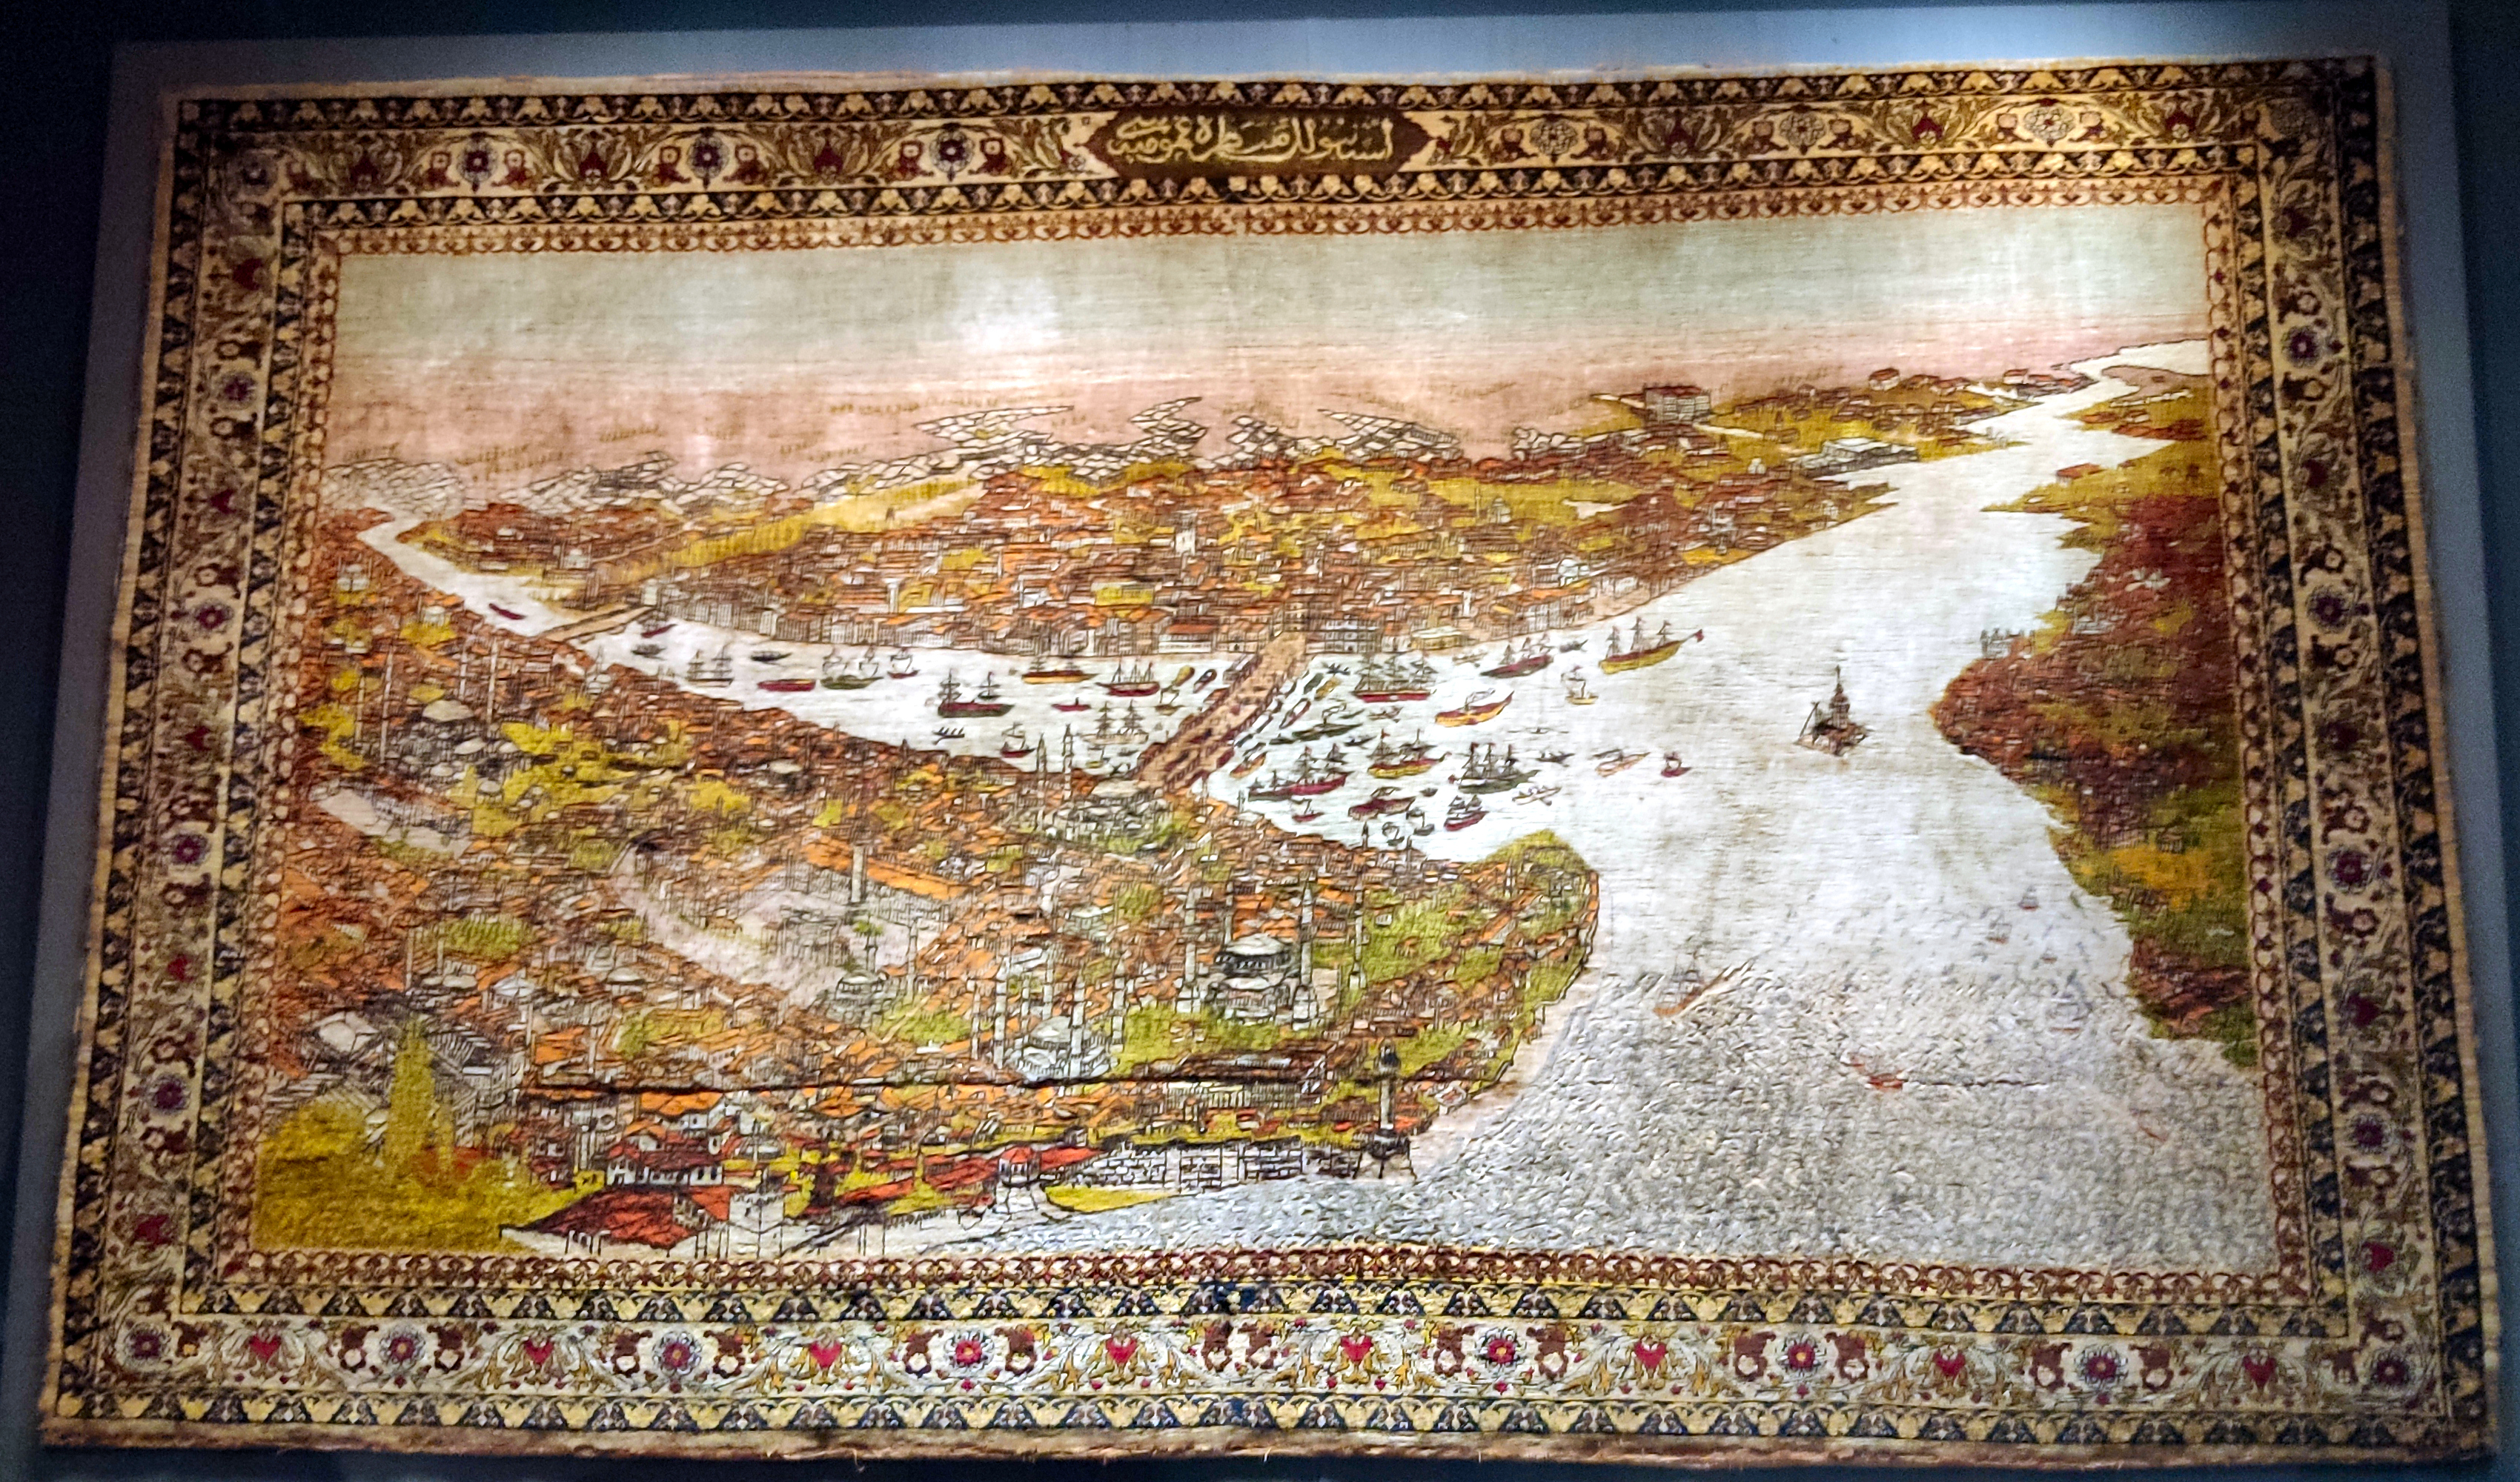
\includegraphics[height=0.4\textheight,width=0.9\linewidth]{assets/istanbul_view.jpg}
    \caption{İstanbul'un Manzara-i Umûmiyesi}
    \label{fig:istanbul_view}
\end{figure}
\indent \textit{İstanbul'un Manzara-i Umûmiyesi} adlı eserin altında Haliç'i ve İstanbul Boğazı'nı kapatan zincirin bir parçası sergilenmektedir. Zincir uygulaması, Bizans döneminde Haliç'i savaş gemilerine kapatmak için kullanılan bir uygulamaydı. Osmanlılar da İstanbul'un fethinden sonra, Sarayburnu ile Haliç arasını bu zincirle kapatarak, Kız Kulesi'nde kurulanbir daire ile gümrük vergisi toplama uygulamasını bir süre uygulamışlardır. Ticarete gelen gemiler Kız Kulesi'ne yanaşarak gerekli işlemleri tamamladıktan sonra Haliç'e giriş yapmaktaydı. Bir deprem sonrası Kız Kulesi'nin zarar görmesinden dolayı bu uygulama 17. yüzyılda kalkmıştır.